\documentclass{llncs}
\usepackage{fullpage}

%load needed packages
\usepackage{graphicx}
\usepackage{array}
\usepackage{booktabs}
\usepackage[utf8]{inputenc}



\begin{document}

\title{APPLICATION OF CLUSTERING METHODS TO
	SPORULATION YEAST MICROARRAY DATA}

\author{Diego De Pablo}
\institute{\email{depablodiego@uma.es} \\
Health Engineering. Málaga University.}

\maketitle 

\vspace{1cm} % Space down the title

\textit{Italic paragraph. Lorem ipsum dolor sit amet, consectetur adipiscing elit, sed do eiusmod tempor incididunt ut labore et dolore magna aliqua. Ut enim ad minim veniam, quis nostrud exercitation ullamco laboris nisi ut aliquip ex ea commodo consequat. Duis aute irure dolor in reprehenderit in voluptate velit esse cillum dolore eu fugiat nulla pariatur. Excepteur sint occaecat cupidatat non proident, sunt in culpa qui officia deserunt mollit anim id est laborum.}

% This is a comment


\section{Introduction}


The aim of this study is to apply clustering techniques to a DNA microarray dataset of \textit{Saccharomyces cerevisiae} gene expression during sporulation, and compare the results with those from a separate analysis.


\subsection*{Temporal Patterns in Gene Expression During Sporulation}

Gene expression during sporulation follows distinct temporal patterns, observe the figure \ref{fig:Sporlutation}, reflecting specific cellular events \cite{chu1998}. These include:
\begin{itemize}
	\item \textbf{Metabolic Early:} Rapid induction at t0.
	\item \textbf{Early I and II:} Sustained expression from t0.5 to t2.
	\item \textbf{Early-Middle:} Peak expression around t5.
	\item \textbf{Middle:} Activation between t5 and t7, related to meiosis.
	\item \textbf{Mid-Late:} Increased expression from t7 to t9, linked to spore wall formation.
	\item \textbf{Late:} Induction between t9 and t11.5, associated with spore maturation.
\end{itemize}

\begin{figure}[h!]
	\begin{center}  % Usamos el entorno 'center'
		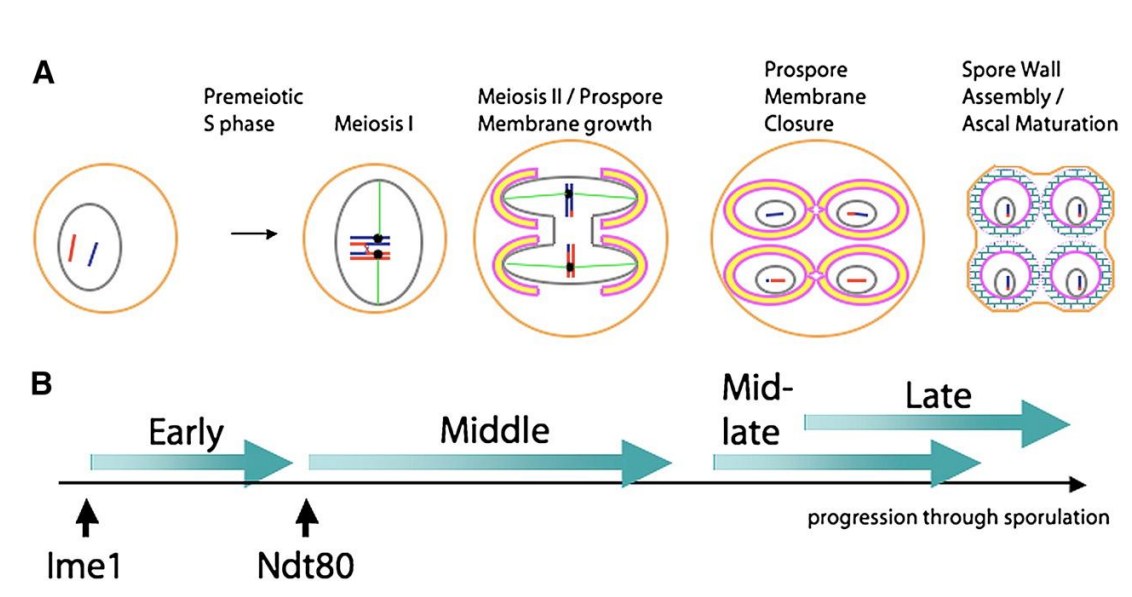
\includegraphics[width=0.6\textwidth]{images/sporlutation.png}
		\caption{A representation of the process of sporulation in budding yeasts}
		\label{fig:Sporlutation}
	\end{center}
\end{figure}

By utilizing DNA microarrays encompassing a significant portion of key genes, we can comprehensively investigate temporal gene expression patterns throughout the process of meiotic spore formation. However, this technique generates large datasets of unlabeled gene expression data, making pattern identification challenging. The abundance of expression levels for hundreds of genes at different time points presents an ideal scenario for applying clustering algorithms to uncover meaningful gene groups and understand the underlying transcriptional regulatory mechanisms.\cite{datta2003}

\subsection*{Application of Clustering Techniques to Analyze Sporulation Data}

While hierarchical clustering (UPGMA) with correlation distance has been a popular choice in microarray studies (at least the begginnings of this century), it's important to recognize the diverse range of clustering algorithms available in pattern recognition and statistics. To classify genes based on their temporal expression profiles during yeast sporulation, we will employ various clustering algorithms, including hierarchical clustering, K-means, self-organizing maps (SOM), and Diana. This comparative analysis aims to identify distinct gene expression patterns and gain insights into the underlying transcriptional regulatory mechanisms.\cite{datta2003}




\section{description of the methods}

Clustering methods The following clustering techniques were considered.


\begin{itemize}
	\item \textbf{Hierarchical Clustering with Correlation:} Hierarchical clustering with correlation is a method that groups data into a hierarchical structure rather than assigning a fixed number of clusters beforehand. It starts with each data point as a separate cluster and gradually merges the closest clusters until a single cluster remains.\cite{guess2002}
	
	\begin{itemize}
		\item \textbf{Algorithm:} The "average" method is used to calculate the distance between clusters. This method computes the average distance between points in one cluster and points in the other cluster.\cite{datta2003}
		
		\item \textbf{Common Method:} This approach, known as UPGMA, is a popular and straightforward method for hierarchical clustering.\cite{datta2003}
		
		\item \textbf{Distance Metric:} The distance between genes is calculated using a correlation-based measure, where a higher correlation indicates greater similarity between the gene expression profiles.\cite{datta2003}
	\end{itemize}
	
	
		
		\item \textbf{K-means Clustering:} Clustering is an unsupervised machine learning technique used to divide a dataset into distinct groups or clusters. Each cluster consists of data points that are more similar to each other than to those in other clusters. K-means is a popular clustering algorithm that partitions data into a predefined number of clusters, represented by centroids. The algorithm works iteratively to assign data points to the nearest centroid, updating centroids based on the mean of the points assigned to each cluster.\cite{steinley2006}
		
		\begin{enumerate}
			\item \textbf{Initialization:} k points are randomly selected from the dataset as initial centroids of the k clusters. These centroids represent the center of each cluster.
			\item \textbf{Assigning Points to Clusters:} Each data point is assigned to the cluster whose centroid is closest. The distance is usually calculated using the Euclidean distance.
			\item \textbf{Updating Centroids:} The positions of the centroids are recalculated as the average of all the points assigned to each cluster.
			\item \textbf{Repetition:} Steps 2 and 3 are repeated until the centroids no longer move significantly or a maximum number of iterations is reached.\cite{steinley2006}
		\end{enumerate}
		
		\item \textbf{Self-Organizing Maps (SOM):} A SOM is an unsupervised neural network that learns to map high-dimensional data onto a low-dimensional grid. It identifies representative prototype vectors and establishes a continuous mapping from the input space to this grid. The grid, often visualized as a 2D map (see Figure \ref{fig:som}), consists of neurons with associated weight vectors. These weight vectors are initially random but converge to represent clusters of similar data points during training.
		
	
\end{itemize}

\begin{figure}[h!]
	\begin{center}  % Usamos el entorno 'center'
		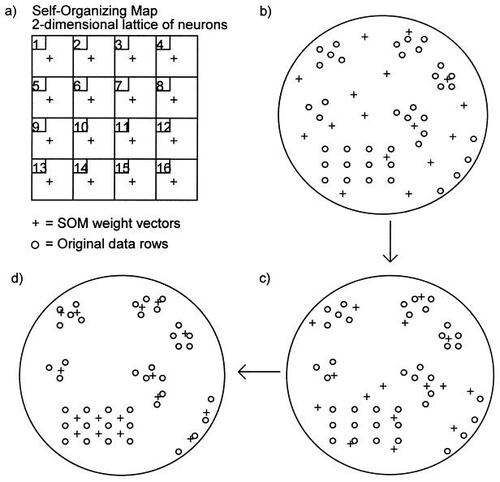
\includegraphics[width=0.45\textwidth]{images/som.jpg}
		\caption{The image illustrates the Self-Organizing Map (SOM) learning process. Panel (a) shows the initial SOM structure, (b) depicts the random initialization of weight vectors, (c) represents an intermediate stage of learning, and (d) shows the final configuration where weight vectors cluster around data points.}
		\label{fig:som}
	\end{center}
\end{figure}

\section{most relevant results obtained comparing both methods}

\textbf{Bold paragraph. Lorem ipsum dolor sit amet, consectetur adipiscing elit, sed do eiusmod tempor incididunt ut labore et dolore magna aliqua. Ut enim ad minim veniam, quis nostrud exercitation ullamco laboris nisi ut aliquip ex ea commodo consequat. Duis aute irure dolor in reprehenderit in voluptate velit esse cillum dolore eu fugiat nulla pariatur. Excepteur sint occaecat cupidatat non proident, sunt in culpa qui officia deserunt mollit anim id est laborum.}
 
 
 \section{Conclusions}
 
 \textbf{Bold paragraph. Lorem ipsum dolor sit amet, consectetur adipiscing elit, sed do eiusmod tempor incididunt ut labore et dolore magna aliqua. Ut enim ad minim veniam, quis nostrud exercitation ullamco laboris nisi ut aliquip ex ea commodo consequat. Duis aute irure dolor in reprehenderit in voluptate velit esse cillum dolore eu fugiat nulla pariatur. Excepteur sint occaecat cupidatat non proident, sunt in culpa qui officia deserunt mollit anim id est laborum.}

\bibliographystyle{plain}  % Puedes cambiar "plain" por el estilo de tu preferencia, como apalike, ieeetr, etc.
\bibliography{bibliography}  % Aquí va el nombre de tu archivo .bib (sin la extensión .bib)
\end{document}
